
\section{Merging}\label{sec:merging}
In this section we will define some approaches and heuristics in order to solve MAPF problems given a \(\tau\) input. The expression ``solving a conflict'' (or similar) will occurs, it however does not represent anything formal; it represents a moment where an approach has a solution to reach a vertex that is after the conflicting vertex, in the sequence of vertices \(\pi\). Thus, it does not mean that no conflict may occur because of the resolution.




\subsection{Sub-graphs}\label{sec:subgraphs}
Approaches in this section are using sub-graphs; one sub-graph is a graph based on \(G\) with the scope of a set of paths \(\gamma\); for every \(\gamma\) in \(\tau\) we have an associated sub-graph \(\mathcal{S}(\gamma)\). In others words, \(n\) agents result in \(n\) sub-graphs. For instance, let an agent \(a_{red}\) and \(a_{blue}\) with their set of paths \(\gamma_{red}\) and \(\gamma_{blue}\) where \(|\gamma_{red}| = 2\) and \(|\gamma_{blue}| = 1\). The result of the decomposition of \(\tau\) in sub-graphs is in figure~\ref{img:from_graph}. 

\begin{figure}[H]
  \centering
  \caption{Decomposition of \(\tau\) in sub-graphs }\label{img:from_graph}
  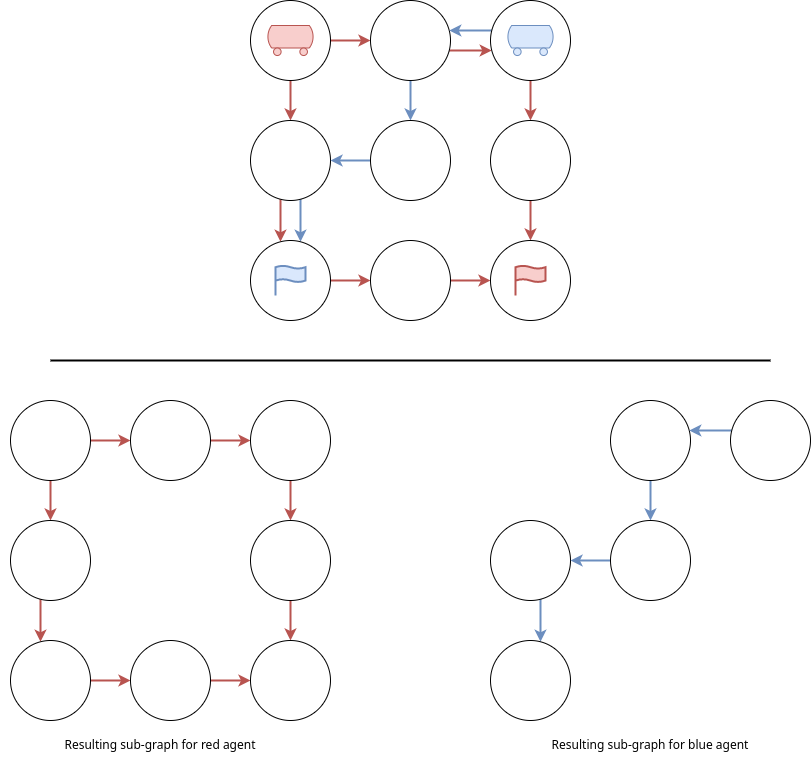
\includegraphics[width=\widthimg]{img/from_graph_to_subgraph.drawio.png}
\end{figure}

Sub-graphs by themselves are not useful, approaches can extend the sub-graphs according to strategies. Intuitively, an ``extension'' represent additional possibilities in order to solve a conflict. 

\subsubsection{Witness solver}

In this section, we will introduce a witness solver; a witness solver (WS) will be the basic solver that aims to solve MAPF instance given a \(\tau\) input. It works as such; it converts the input \(\tau\) in a set of \(n\) graph that are sub-graph of \(G\) as described in section~\ref{sec:subgraphs}. We then have two cases: there is a valid plan made out from \(\tau\) that contains no path-conflict, or there is no valid plan that can be build lot of \(\tau\) directly. In the first case, the merging process will give the valid plan as output, in the second case, the WS will try to solve the instance by using different approaches, strategies or heuristics until finding a valid set of paths that is a valid plan.

The first case occurs if it exists a set \(\{pick(\gamma) | \gamma \in \tau\}\) which correspond to a collection of paths, is conflict-free, we refer to this case as ``straightforward solving''.

\begin{figure}[H]
  \centering
  \caption{Example of instance that is not possible to use straightforward solving}\label{img:heatmap_sf_solving}
  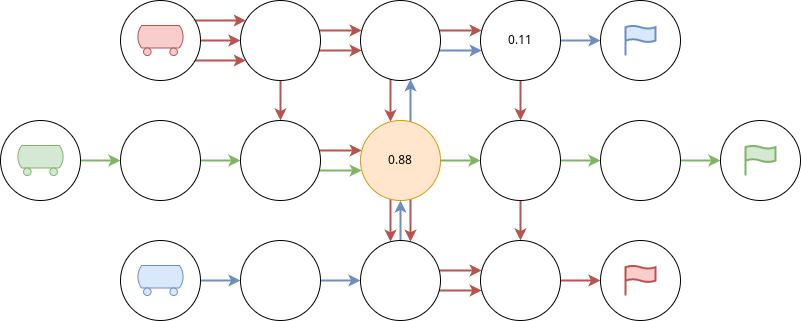
\includegraphics[width=\widthimg]{img/heatmap_sf_solving.drawio.png}
\end{figure}

\begin{figure}[H]
  \centering
  \caption{Example of instance that straightforward solving is at least undetermined}\label{img:heatmap_sf_solving_possible}
  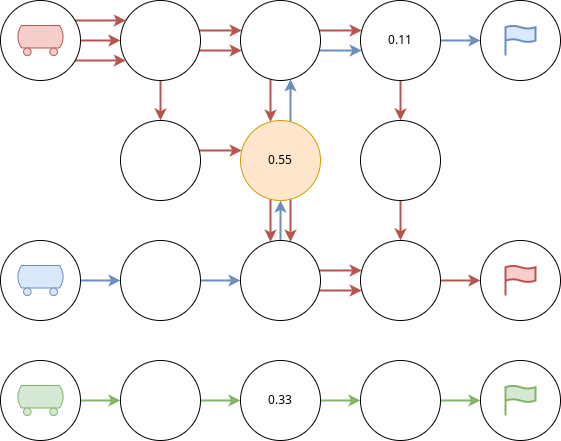
\includegraphics[width=8cm]{img/heatmap_sf_solving_possible.drawio.png}
\end{figure}

\subsubsection{Corridor}\label{sec:corridor}

The corridor approach aims to help the solving process by extending the size of the sub-graph generated by a set of path \(\gamma\). It extends the sub-graph by adding to the sub-graph the direct neighbor vertices (and their associated edges). Applying the corridor extension successively \(x\) times will result of a corridor of level \(x\) for instance:  
\begin{figure}[H]
  \centering
  \caption{Example of corridor}\label{img:corridor}
  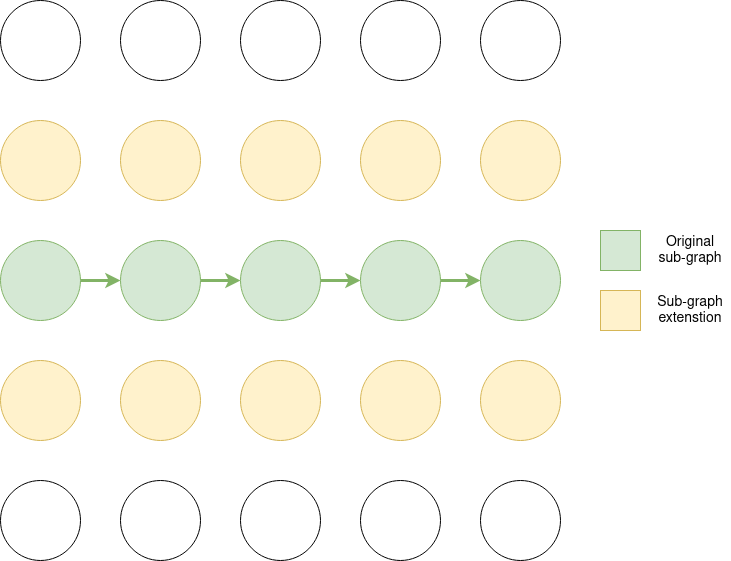
\includegraphics[width=\widthimg]{img/corridor.drawio}
\end{figure}

We can define corridor as such;

\[
 corridor(s,(V,E)) = \{v' | v' \in V, v\in s, (v,v') \in E \}
\] where s represent of set of vertices.

A corridor of \(k\)-level(s) is obtained by recursively use the corridor function \(k\) time on its output: e.g. \(corridor(corridor(vertex(\pi),G))\) represent a 2-levels corridor.
We can assume some elements about this approach; with a big enough \(k\) size the whole graph is covered. Using the witness solver would end up doing classic MAPF. Furthermore, for large instances, a huge part of the extension would probably not be used ending up adding more space search for the witness solver. We can also identify instances where corridor extension would be probably interesting to use when the ``dodge'' movement required to solve a conflict situated in the graph ``far away'' (the figure~\ref{img:systemetic_instance} is an example; informally, it requires the agents to move away from their original paths) from where the conflict occurred. We can also assume that a set of distant paths would be an interesting set to work with; it potentially limits the number of ``overlapping'' vertices that would be added by the extension, see example shown in figure~\ref{img:case_corridor}. Also, corridors may work better on low density instances and low number of conflicts and potential conflict since it is not adding so much depth of possible movement.

In practice, we can create corridor only for path that have a path conflict, we can also choose to create corridor only for one of the two agent involved in a conflict.


\begin{figure}[H]
  \centering
  \caption{Most Distant paths and corridor extension}\label{img:case_corridor}
  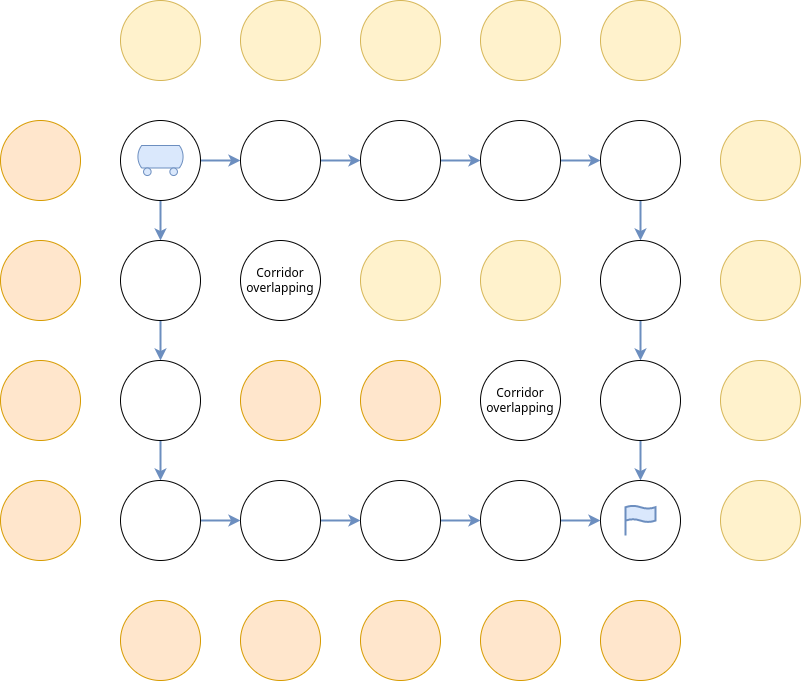
\includegraphics[width=\widthimg]{img/case_corridor.drawio.png}
\end{figure}


\subsubsection{Diamond extension}

The diamond extension aims to extend the sub-graph by adding diamonds of vertices around potential conflict or plan conflict. As shown in figure~\ref{img:diamond}, we can see different levels of diamond extension which will increase the size of the sub-graph, by extension the possibilities in order to solve the conflict.
\begin{figure}[H]
  \centering
  \caption{Example of diamond of size 1 and 2}\label{img:diamond}
  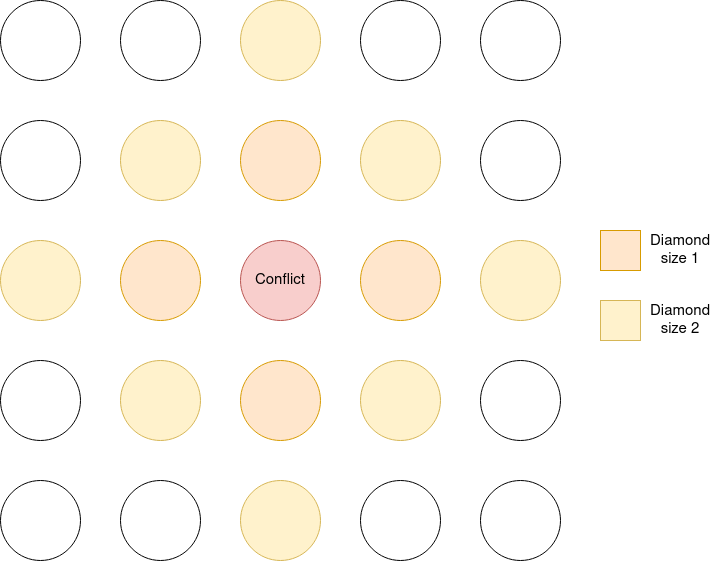
\includegraphics[width=\widthimg]{img/diamond.drawio.png}
\end{figure}

As described for the corridor instance, having a \(k\) as diamond size too big would end up covering the whole graph. This approach would probably work fine with a relatively small \nameref{sec:conflict_window}; having all conflicts concentrated in area of the graph would allow small size of the diamond extension, which reduce the space search. The instance represented in figure~\ref{img:diamond_case}, has a ``small'' conflict-window. While solving this instance (or this kind of instance, a lot of robots, small conflict window) we can easily imagine that solving the conflicts issued by the IPF would create other conflicts but still in the same area. In consequences, diamond extension seems appropriate since the extension is covering also close area around conflicts. 
\begin{figure}[H]
  \centering
  \caption{Example of diamond extension interesting case }\label{img:diamond_case}
  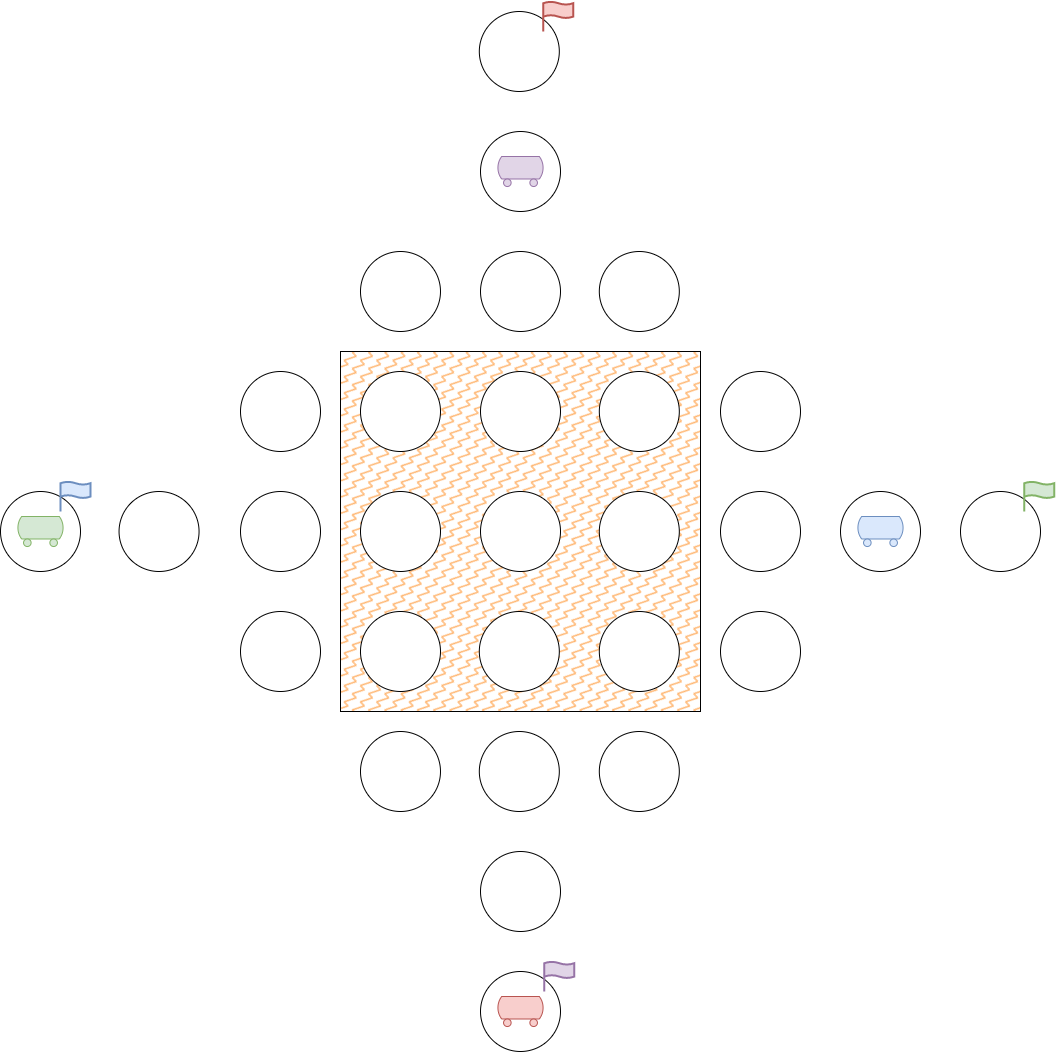
\includegraphics[width=7cm]{img/diamond_extension_case_example.drawio.png}
\end{figure}

From the properties described in section~\ref{sec:ipf}, we can argue that paths that have few bendings would work better for the diamond extension; a higher proportion of the extension (of size higher than 1) will already be in the original paths. Furthermore, contrary to the corridor extension, whenever the proportion of conflict is low compared to the length of the path, diamond extension would probably work better e.g. figure\ref{img:diamond_vs_corridor}, based on section~\ref{sec:corridor} and figure~\ref{img:corridor} the proportion of the sub-graph that is not used is way higher for the diamond extension.

\begin{figure}[H]
  \centering
  \caption{Example of case where diamond extension would work but not corridor extension}\label{img:diamond_vs_corridor}
  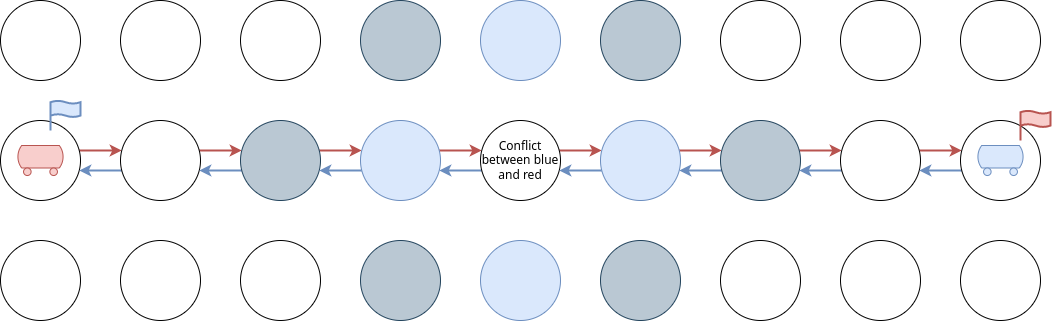
\includegraphics[width=\widthimg]{img/diamond_vs_corridor.drawio.png}
\end{figure}





\subsubsection{Systematic extension}

Approach presented above are not complete and aim to reduce the space search or computation time at the probable cost of optionality. Furthermore, we can imagine instances where both approaches would not work, or require too much computation time. In the case represented on figure~\ref{img:systemetic_instance}, considering that \(\tau\) contains for both agent one shortest path, it is easy to tell that both heuristics on this kind of instances would not work decently because it would require that the extension covers the whole graph.

\begin{figure}[H]
  \centering
  \caption{Example instance that are more complex to solve}\label{img:systemetic_instance}
  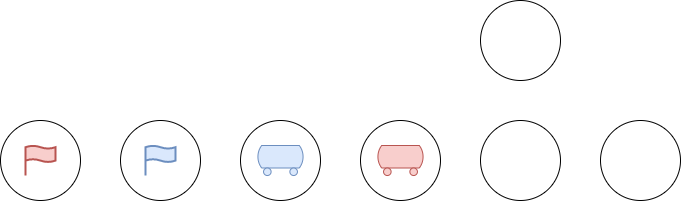
\includegraphics[width=\widthimg]{img/systematic_instance.drawio.png}
\end{figure}

We can use solving strategies described in paper~\cite{husvobbass22a,husvobbass22b}. These paper introduce four different strategies; Baseline Strategy, Makespan-add Strategy, Prune-and-cut strategy and the Combined strategy. For short, these strategies are using a \(k-restricted graph\) which is similar to sub-graph; it takes a shortest path \(SP\) to define a subgraph, it also adds ``vertices that are at most distance \(k\) away from some vertex in \(SP\)". The main idea is to add vertices and/or raise the makespan and see if a solution exist. According to the benchmarks, the Combined strategy seems to be most successful.

\subsubsection{Improving subgraphs with heatmaps}

An advantage of the subgraphs approach is that the approach can work till the subgraph contains the initial and final position and is connected. We can then, instead of increasing its size as we proposed before, prune part of the graph. To do so, we can aim specific vertices of the graph that can be identified using heatmap (see~\ref{sec:heatmap}). In a way, we can try to reduce \(\Phi\) values of the global heatmap by removing some vertices of subgraphs. We can imagine different criteria that would be deciding which vertex can, or should be pruned, for instance we can select vertices of the subgraph that have a high \(\Phi\) value but a low \(\phi\) one. In other words, removing vertices that are, for an agent not ``essential'' because not used multiple times, but used by other agents. 

On the other hand, heatmap can be used to tune the different approaches we described before. For instance, we can apply bigger diamond extension on a vertex that have a conflict and a high \(\Phi\) value, or even selecting which agent the extension would be applied on. 

\subsection{Solving with heatmap}

\subsubsection{Straightforward solving}
We described succinctly "straightforward solving", however, the process of picking these paths may be costly due to the exponential numbers of combination. We can use heatmap as a preprocessing work or as a solving technique ; from a global heatmap, we can directly tell from the paths if a straightforward solving is not possible if the following equation is true; 
\[ 
  \Phi(v,t,\tau) > \frac{ \sum^{\pi \in \gamma}{(1 \text{ if } v = \pi(t) \text{, else } 0)}}{|A|}
\] 
with \(|A| > 1\), for any vertex \(v\), at any time \(t\). The following figure~\ref{img:heatmap_sf_solving} shows an example where the straightforward solving is decided from the heatmap; the orange vertex as a \(\Phi\) value superior to \(3/4\). On the other side, the figure~\ref{img:heatmap_sf_solving_possible} show the opposite case.

\subsubsection{Guiding the agents}

We described above strategies working with sub-graphs, however we can use \(\tau\) in other way; guiding the agents. \(\tau\) serves then the purpose of indicates where agents can or should be. A possible representation is the global heatmap, by valuing the graph the agents evolve on, we can build path for an agent that are not contained in its \(\gamma\). The global idea is to make the agent follow the lowest values of the global heatmap to avoid conflict. Since the heatmap is defined per time step, we are guarantee that the agents will move towards their goal position.

The process of solving must handle at least two scenarios: one where no conflicts arise while selecting vertices, and on another side, selecting the lowest heat value would result in a conflict at the next step, with no other options available. The first scenario represents normal behavior, where each step involves selecting the most appealing vertex. The second scenario involves proposing different approaches to address the absence of options available in the heatmap to avoid conflict. If the next conflict involves a vertex, one of the agents creating the conflict can wait. If the conflict is an edge conflict, one of the agents must move to an uncovered vertex. However, this is not always feasible, and in such cases, heuristics must be applied since the heatmap alone does not seem to provide a solution.

One notable feature of the heatmap approach is that it is able to take into account paths of varying lengths; contrary to subgraph approach, any additional path of any length has an impact on the values of the heatmap. On the other hand, we can imagine paths (of any length) where all vertices in their sequence are already included in the subgraph.



